\begin{longversion}
%
%
The data for the gold standard was collected via the KrdWrd Add-on (cf.~\ref{sec:addon})
as an homework assignment (cf.~\ref{sec:assignment}) for a Computational Linguistics class,
which is a second year undergraduate Cognitive Science class at the University of Osnabr\"{u}ck.
The Annotators were introduced to the KrdWrd Annotation Guidelines (cf.~\ref{sec:guidelines}) by means of the KrdWrd Tutorial (cf.~\ref{sec:tutorial}), and 
were supposed to work independently (e.g.~from their home PC) though, could have sat near each other. 
However, we did take precautions against na\"{i}ve copying by enforcing authentication for the users with their student accounts,
hiding other users' results, and
serving random pages for tagging -- thus, even if students were exchanging information it could rather have been about the assignment and the tagging in general than a specific Web site in particular.

\subsection{Initial Observations}
From 100 student subscribed to the class 69 installed the Add-on and submitted at least one page (not necessarily a tagged one, though\ldots).
This was also about the ratio of students who took the final exam for this course hence, we can say that almost every students seriously interested in finishing this class also took the homework assignment.

The majority of submissions came within the last 4 days of the period of time they were granted to finish the assignment -- with a major peak at the last day;
which, according to all we know, is quite common.
This has probably also led to only very few people making use of the re-submit feature, i.e.~continuing or modifying an already submitted page.

The possibility to interact with the KrdWrd Team, e.g.~to solve installation problems, or to exchange information via an e-Mail list we had set up for this purpose was rarely used (cf.~\url{https://krdwrd.org/trac/mail/threads}).
The few reported problems however, led to some beneficial improvements of the documentation.

\paragraph{Our initial Data Set} (before further clean-up):
228 Web pages, consisting of almost 440,000 words and over 2.6 million characters, were independently processed by
69 users who submitted 
1767 results (re-submits for a page counted only once), which is an average of 7.75 submissions per page. 


% What, (Why,) How, Result
\subsection{The KrdWrd App: Annotations Merging Mode}

The KrdWrd App in merging mode compares the initially grabed \emph{master} with the user submitted results and, for every text node in the DOM tree, computes a majority vote and assigns this as the gold standard tag to the node of a newly created document. 

The process is carried out offline on the server:
the input is one URL of a master document and the URLs of the respective user submitted results.
After reading all documents the DOM trees of all documents are traversed top-down and tags along the traversal are propagated further down as long as, 
no more specific tag is encountered,
i.e.~a tag can not overwrite another one further down the path but is \emph{pushed down} as far as possible (cf.~figure \ref{fig:propagation} for an illustration).
At the end of each path in the tree the assigned tags are counted.
After having traversed all documents a sanity check is carried out\footnote{
We also implemented another sanity check namely, to check whether the textual content in the nodes is identical but dropped this condition -- mainly because the few encounters were false positives and it had negative impact on performance as well.
} \footnote{
The overall handling of JavaScript is not satisfactory.
To address the diversions between submits occurring after dynamic client-side JavaScript execution on different clients, the Add-on could hook into the node creation and clone processes.
They could be suppressed entirely or newly created nodes could grow a special id tag to help identifying them later.
} namely, are there documents which still have unseen nodes, or are there documents which had less nodes than the master document? 
In either case, these submissions are discarded from further processing.

The remaining submissions are taken into account for the majority vote on each node of the master document.
Another document is generated, which includes the resulting tags.

\begin{figure}[htb]
    \centering
    \begin{minipage}[c]{.9\textwidth}
        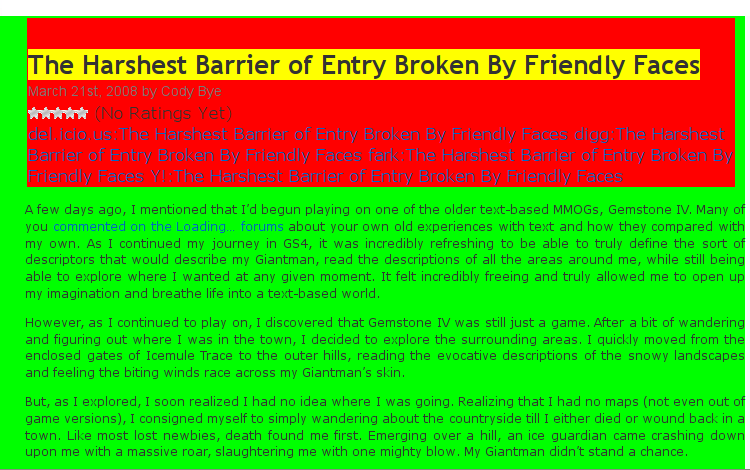
\includegraphics[width=.48\textwidth,keepaspectratio]{preprop}
        \hfill
        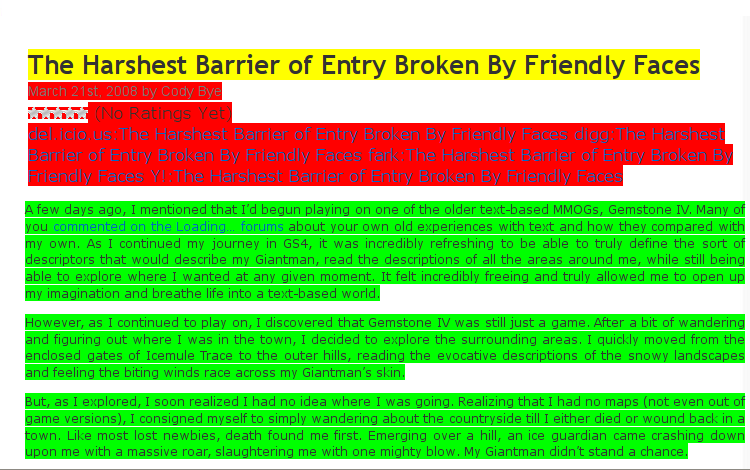
\includegraphics[width=.48\textwidth,keepaspectratio]{postprop}
    \end{minipage}
    \caption{On the left is the un-propagated page with major parts having been tagged green and red. On the right is the propagated version where the green has been pushed down into the text nodes; the same holds for red but note that the heading in yellow has not been overwritten.}
    \label{fig:propagation}
\end{figure}


% What, (Why,) How, Result
\subsection{Merge Analysis}

Before we started to analyse the results of the merging process we excluded the results of one user who had only submitted one page. 
Then, the merging process revealed the following problematic cases (usually by rejecting user results on grounds of the sanity check): 
%2: 690, 870
2 pages with no results left to merge,
%3: 708, 715, 908 (708:bad, rest ok)
3 pages with only one result to merge,
%2: 714, 720 (714: poor, 720: bad)
2 more pages with only two result to merge,
%1: 746
1 page with four results to merge, and 
%1:?
1 page that could not be merged due to an error in our application\footnote{We fixed the error but this rendered the submitted pages unusable -- newly submitted pages will be mergable.}.
We also excluded all these cases from further processing (cf.~figure \ref{fig:submsperpage}).

\fig{.9}{submsperpage_hist}{Number of Pages with x Submissions - the dividing line at \emph{5 Submissions} shows the cut-off, i.e.~pages with less then 5 Submissions were excluded from further processing. The observant reader may notice that we said the annotations were evenly distributed: this is the case, now. We had not turned on this feature when we started collecting the data, however.}{fig:submsperpage}

We continued to do a plausibility check for the submitted results:
we computed a \emph{tag-bias} for each user, where we compared each user's tendency to chose a tag for a node with the actual winning tags for nodes. 
This computation revealed 
% 4: 14, 34, 31, 74
4 cases in which users showed strong biases towards certain tags\footnote{Manual inspection of these cases showed that the users obviously only wanted to raise their tagged-pages count and therefore, just tagged very few nodes -- typically high up in the DOM tree -- which were then propagated downwards.}.
We also excluded all results from these users.

% BADUIDS=(14 31 34 73 74)
\paragraph{The resulting and final Data Set:}
219 Web pages, consisting of more than 420,000 words and over 2.5 million characters, were independently processed by
64 users who submitted 
1595 results (re-submits for a page counted only once), which is an average of 7.28 submissions per page. 

\noindent \newline
We continued our analyses of this new data at hand, and looked into the timestamps we collected for the submissions:
therefore, we summed up all the deltas between two submissions for each user and calculated the duration each user \emph{saw} a single page;
then, we computed a reasonable upper bound for how log a submit action might take,
i.e.~the hypothesis was that page-view times longer than a certain amount of time were actually breaks.
To this end, we detected outliers\footnote{This is quite standard: $x$ values outside the range $Q1 - 1.5*IQR < x < 1.5*IQR + Q3$ were considered outliers.} and discarded \emph{all} respective submissions (the calculated\cite{r-project} result was 700s).

The calculated time data suggests that:
\begin{itemize}
\item the majority of users spent between 56 and 88 minutes on the assignment with an average of 71 minutes (cf.~figure \ref{fig:timespentonassignment} for details), 
\item average per-page annotation time drops below three minutes (cf.~figure \ref{fig:timespentonpage}), and
\item the first pages after the tutorial are still more challenging than later ones (cf.~\ref{fig:sequencedelta}).
\end{itemize}

\fig{.9}{timespentonassignment}{Time in Minutes spent by y Users on the Assignment, i.e.~how much Time did a User interact with the Add-on to tag her share of the Canola Corpus.}{fig:timespentonassignment}
% Min. 1st Qu.  Median    Mean 3rd Qu.    Max. 
% 11.92   56.03   69.52   70.64   88.10  140.70

\fig{.9}{timespentonpage}{Minutes spent on a single Page accross all annotations of the Canola corpus.}{fig:timespentonpage}
% Min. 1st Qu.  Median    Mean 3rd Qu.    Max. 
% 28.6   121.9   172.2   168.5   200.0   324.2 

\fig{.55}{sequencedelta}{Smoothened average of differences in seconds between annotation times of all users at Position x in their specific sequences of Web Pages and the mean of all other users who processed identical pages at a later time in their respective sequences.}{fig:sequencedelta}


%length:
% - num word/nodes does not correlate to time for page - only for quite short documents
% - long time spent on documents: long /rendered/ documents - but also one of the quickest and best tagged documents is among them\ldots
%
% 716(took the longest) 697 696 815 774 ||  888 765 769 910 767(shortes)
% https://krdwrd.org/pages/bin/view/[NUMBER]

%\subsection{Agreement and Disagreement Analysis of Annotations}

\fig{.9}{pagesperuser}{Aggregated counts for the Number of Users who processed \emph{at least} x Number of Pages. Note the two steps at 15 and 25 pages, which correspond to the obligatory and the optional number of pages in the assignment. Also note that there were quite many students who went far beyond the requirement for the assignment.}{fig:pagesperuse}

For the overall inter-coder agreement of the remaining submissions we calculated Fleiss's multi-$\pi$ as layed out in \cite{ArtsteinPoesio2008}: for each Web page the remaining submissions were set as coders, and the tagged DOM nodes as items -- the three categories were fixed.
This resulted in an average inter-coder agreement over all pages of 0.85 (cf.~\ref{fig:agreementonpages}), which we think is -- at least -- substantial.
Considering that these submissions were the basis for the merge process we believe that the Canola Gold Standard Corpus is a solid basis for further processing.
Furthermore, this metric could be used for comparison of cleaning results in general -- maybe normalised for the number of words or characters per DOM node.

\fig{.9}{agreementonpages}{Inter-coder agreement between submissions for pages over the Canola corpus.}{fig:agreementonpages}
% Min. 1st Qu.  Median    Mean 3rd Qu.    Max. 
% 0.4166  0.7508  0.8585  0.8260  0.9246  1.0000

\paragraph{Remark:} we looked into the pages at the lower end of the agreement spectrum and found that they tended to be quite long and were often discussion forum pages, i.e.~with many alterations in the tags that were to assign. Given that similar shorter pages achieved better results, it seems that even our already quite low boundary of 6,000 words per page resulted in pages that were frustrating to process.
%
%
\end{longversion}

